\documentclass[12pt,a4paper]{article}
\usepackage[utf8]{inputenc}
\usepackage[T1]{fontenc}
\usepackage[english]{babel}
\usepackage[top=2cm,bottom=2cm,left=2.5cm,right=2.5cm]{geometry}
\usepackage{amsmath,amssymb,amsthm}
\usepackage{enumitem}
\usepackage{tcolorbox}
\usepackage{tikz}
\usepackage{pgfplots}
\pgfplotsset{compat=1.18}
\usepackage{hyperref}

\tcbuselibrary{breakable,skins}

% Exercise/Solution environment
\newcounter{exercise}[section]
\newenvironment{exercise}{\refstepcounter{exercise}\par\medskip\noindent\textbf{Exercise \thesection.\theexercise.}}{\par\medskip}

\newtcolorbox{solution}{
    colback=green!5!white,
    colframe=green!60!black,
    fonttitle=\bfseries,
    title=Solution,
    breakable,
    before skip=6pt,
    after skip=6pt
}

\title{\textbf{MathTrackX: Exercises and Solutions}\\[0.5cm]
\large Polynomials, Functions and Graphs\\
Based on University of Adelaide Curriculum}
\author{SOLTANI Achraf}
\date{\today}

\begin{document}

\maketitle
\tableofcontents
\newpage

%=============================================================================
\section{Week 1: Numbers}
%=============================================================================

\subsection{Number Types}

\begin{exercise}
Classify each number as natural ($\mathbb{N}$), integer ($\mathbb{Z}$), rational ($\mathbb{Q}$), or irrational. Select the most specific category.
\begin{enumerate}[label=(\alph*)]
    \item $-7$
    \item $\frac{22}{7}$
    \item $\sqrt{16}$
    \item $\pi$
    \item $0.\overline{45}$
    \item $\sqrt{5}$
\end{enumerate}
\end{exercise}

\begin{solution}
\begin{enumerate}[label=(\alph*)]
    \item $-7$: \textbf{Integer} ($\mathbb{Z}$) --- negative, so not natural
    \item $\frac{22}{7}$: \textbf{Rational} ($\mathbb{Q}$) --- fraction of integers
    \item $\sqrt{16} = 4$: \textbf{Natural} ($\mathbb{N}$) --- positive whole number
    \item $\pi$: \textbf{Irrational} --- non-repeating, non-terminating decimal
    \item $0.\overline{45}$: \textbf{Rational} ($\mathbb{Q}$) --- repeating decimal = $\frac{45}{99} = \frac{5}{11}$
    \item $\sqrt{5}$: \textbf{Irrational} --- cannot be expressed as a fraction
\end{enumerate}
\end{solution}

\begin{exercise}
Convert the repeating decimal $0.\overline{36}$ to a fraction in lowest terms.
\end{exercise}

\begin{solution}
Let $x = 0.\overline{36} = 0.363636\ldots$

Multiply by 100: $100x = 36.363636\ldots$

Subtract: $100x - x = 36$

$99x = 36$

$x = \frac{36}{99} = \boxed{\frac{4}{11}}$
\end{solution}

\subsection{Arithmetic}

\begin{exercise}
Simplify each expression:
\begin{enumerate}[label=(\alph*)]
    \item $\frac{3}{4} + \frac{5}{6}$
    \item $\frac{7}{8} - \frac{2}{3}$
    \item $\frac{2}{5} \times \frac{15}{8}$
    \item $\frac{3}{4} \div \frac{9}{16}$
\end{enumerate}
\end{exercise}

\begin{solution}
\begin{enumerate}[label=(\alph*)]
    \item $\frac{3}{4} + \frac{5}{6} = \frac{9}{12} + \frac{10}{12} = \boxed{\frac{19}{12}}$

    \item $\frac{7}{8} - \frac{2}{3} = \frac{21}{24} - \frac{16}{24} = \boxed{\frac{5}{24}}$

    \item $\frac{2}{5} \times \frac{15}{8} = \frac{30}{40} = \boxed{\frac{3}{4}}$

    \item $\frac{3}{4} \div \frac{9}{16} = \frac{3}{4} \times \frac{16}{9} = \frac{48}{36} = \boxed{\frac{4}{3}}$
\end{enumerate}
\end{solution}

\begin{exercise}
Evaluate using the correct order of operations:
\begin{enumerate}[label=(\alph*)]
    \item $2 + 3 \times 4 - 1$
    \item $(2 + 3) \times (4 - 1)$
    \item $12 \div 4 + 2^3 \times 3$
    \item $\frac{6 + 2 \times 4}{7 - 3}$
\end{enumerate}
\end{exercise}

\begin{solution}
\begin{enumerate}[label=(\alph*)]
    \item $2 + 3 \times 4 - 1 = 2 + 12 - 1 = \boxed{13}$

    \item $(2 + 3) \times (4 - 1) = 5 \times 3 = \boxed{15}$

    \item $12 \div 4 + 2^3 \times 3 = 3 + 8 \times 3 = 3 + 24 = \boxed{27}$

    \item $\frac{6 + 2 \times 4}{7 - 3} = \frac{6 + 8}{4} = \frac{14}{4} = \boxed{\frac{7}{2}}$
\end{enumerate}
\end{solution}

\subsection{Inequalities and Intervals}

\begin{exercise}
Solve each inequality and express the answer in interval notation:
\begin{enumerate}[label=(\alph*)]
    \item $3x - 5 > 7$
    \item $-2x + 4 \leq 10$
    \item $5 - 3x < 2x + 10$
    \item $\frac{x}{2} - 3 \geq 1$
\end{enumerate}
\end{exercise}

\begin{solution}
\begin{enumerate}[label=(\alph*)]
    \item $3x - 5 > 7 \Rightarrow 3x > 12 \Rightarrow x > 4$

    Answer: $\boxed{(4, \infty)}$

    \item $-2x + 4 \leq 10 \Rightarrow -2x \leq 6 \Rightarrow x \geq -3$ (reverse inequality!)

    Answer: $\boxed{[-3, \infty)}$

    \item $5 - 3x < 2x + 10 \Rightarrow -5x < 5 \Rightarrow x > -1$

    Answer: $\boxed{(-1, \infty)}$

    \item $\frac{x}{2} - 3 \geq 1 \Rightarrow \frac{x}{2} \geq 4 \Rightarrow x \geq 8$

    Answer: $\boxed{[8, \infty)}$
\end{enumerate}
\end{solution}

\begin{exercise}
Express each statement using interval notation:
\begin{enumerate}[label=(\alph*)]
    \item $x$ is greater than $-2$ and less than or equal to $5$
    \item $x$ is at most $3$
    \item $x$ is at least $-1$ but less than $4$
\end{enumerate}
\end{exercise}

\begin{solution}
\begin{enumerate}[label=(\alph*)]
    \item $-2 < x \leq 5$: $\boxed{(-2, 5]}$
    \item $x \leq 3$: $\boxed{(-\infty, 3]}$
    \item $-1 \leq x < 4$: $\boxed{[-1, 4)}$
\end{enumerate}
\end{solution}

\begin{exercise}
Evaluate:
\begin{enumerate}[label=(\alph*)]
    \item $|{-8}| + |3|$
    \item $|5 - 12|$
    \item $|{-2}| \times |{-7}|$
\end{enumerate}
\end{exercise}

\begin{solution}
\begin{enumerate}[label=(\alph*)]
    \item $|-8| + |3| = 8 + 3 = \boxed{11}$
    \item $|5 - 12| = |-7| = \boxed{7}$
    \item $|-2| \times |-7| = 2 \times 7 = \boxed{14}$
\end{enumerate}
\end{solution}

%=============================================================================
\section{Week 2: Linear Functions}
%=============================================================================

\subsection{Coordinate Plane and Functions}

\begin{exercise}
Plot and identify the quadrant for each point:
\begin{enumerate}[label=(\alph*)]
    \item $(3, -2)$
    \item $(-4, 5)$
    \item $(-1, -3)$
    \item $(0, 4)$
\end{enumerate}
\end{exercise}

\begin{solution}
\begin{enumerate}[label=(\alph*)]
    \item $(3, -2)$: \textbf{Quadrant IV} (positive $x$, negative $y$)
    \item $(-4, 5)$: \textbf{Quadrant II} (negative $x$, positive $y$)
    \item $(-1, -3)$: \textbf{Quadrant III} (both negative)
    \item $(0, 4)$: \textbf{On the $y$-axis} (not in any quadrant)
\end{enumerate}
\end{solution}

\begin{exercise}
For $f(x) = 3x - 5$, find:
\begin{enumerate}[label=(\alph*)]
    \item $f(0)$
    \item $f(2)$
    \item $f(-1)$
    \item The value of $x$ when $f(x) = 7$
\end{enumerate}
\end{exercise}

\begin{solution}
\begin{enumerate}[label=(\alph*)]
    \item $f(0) = 3(0) - 5 = \boxed{-5}$
    \item $f(2) = 3(2) - 5 = 6 - 5 = \boxed{1}$
    \item $f(-1) = 3(-1) - 5 = -3 - 5 = \boxed{-8}$
    \item $3x - 5 = 7 \Rightarrow 3x = 12 \Rightarrow x = \boxed{4}$
\end{enumerate}
\end{solution}

\subsection{Slope and Linear Equations}

\begin{exercise}
Find the slope of the line passing through each pair of points:
\begin{enumerate}[label=(\alph*)]
    \item $(1, 3)$ and $(4, 9)$
    \item $(-2, 5)$ and $(3, -5)$
    \item $(0, 4)$ and $(6, 4)$
    \item $(3, 1)$ and $(3, 7)$
\end{enumerate}
\end{exercise}

\begin{solution}
Using $m = \frac{y_2 - y_1}{x_2 - x_1}$:
\begin{enumerate}[label=(\alph*)]
    \item $m = \frac{9 - 3}{4 - 1} = \frac{6}{3} = \boxed{2}$
    \item $m = \frac{-5 - 5}{3 - (-2)} = \frac{-10}{5} = \boxed{-2}$
    \item $m = \frac{4 - 4}{6 - 0} = \frac{0}{6} = \boxed{0}$ (horizontal line)
    \item $m = \frac{7 - 1}{3 - 3} = \frac{6}{0}$ = \textbf{undefined} (vertical line)
\end{enumerate}
\end{solution}

\begin{exercise}
Write the equation of the line in slope-intercept form ($y = mx + b$):
\begin{enumerate}[label=(\alph*)]
    \item Slope $2$, $y$-intercept $(0, -3)$
    \item Through $(2, 5)$ with slope $-1$
    \item Through $(1, 4)$ and $(3, 10)$
    \item Through $(-2, 3)$ parallel to $y = 4x - 1$
\end{enumerate}
\end{exercise}

\begin{solution}
\begin{enumerate}[label=(\alph*)]
    \item $m = 2$, $b = -3$: $\boxed{y = 2x - 3}$

    \item Using point-slope: $y - 5 = -1(x - 2)$

    $y = -x + 2 + 5 = \boxed{y = -x + 7}$

    \item Slope: $m = \frac{10-4}{3-1} = 3$

    Point-slope: $y - 4 = 3(x - 1)$

    $\boxed{y = 3x + 1}$

    \item Parallel $\Rightarrow$ same slope $m = 4$

    $y - 3 = 4(x + 2)$

    $\boxed{y = 4x + 11}$
\end{enumerate}
\end{solution}

\begin{exercise}
Find the equation of the line perpendicular to $y = \frac{2}{3}x + 1$ passing through $(4, -1)$.
\end{exercise}

\begin{solution}
Perpendicular slope: $m_\perp = -\frac{1}{2/3} = -\frac{3}{2}$

Using point-slope: $y - (-1) = -\frac{3}{2}(x - 4)$

$y + 1 = -\frac{3}{2}x + 6$

$\boxed{y = -\frac{3}{2}x + 5}$
\end{solution}

\begin{exercise}
Find the $x$-intercept and $y$-intercept of $3x - 2y = 12$.
\end{exercise}

\begin{solution}
\textbf{$y$-intercept:} Set $x = 0$:

$-2y = 12 \Rightarrow y = -6$

$y$-intercept: $\boxed{(0, -6)}$

\textbf{$x$-intercept:} Set $y = 0$:

$3x = 12 \Rightarrow x = 4$

$x$-intercept: $\boxed{(4, 0)}$
\end{solution}

%=============================================================================
\section{Week 3: Polynomials}
%=============================================================================

\subsection{Polynomial Basics}

\begin{exercise}
For $P(x) = -2x^4 + 5x^3 - x + 7$, identify:
\begin{enumerate}[label=(\alph*)]
    \item The degree
    \item The leading coefficient
    \item The constant term
    \item $P(0)$
    \item $P(1)$
\end{enumerate}
\end{exercise}

\begin{solution}
\begin{enumerate}[label=(\alph*)]
    \item Degree: $\boxed{4}$
    \item Leading coefficient: $\boxed{-2}$
    \item Constant term: $\boxed{7}$
    \item $P(0) = 7$
    \item $P(1) = -2 + 5 - 1 + 7 = \boxed{9}$
\end{enumerate}
\end{solution}

\begin{exercise}
Expand using special products:
\begin{enumerate}[label=(\alph*)]
    \item $(x + 5)^2$
    \item $(3x - 2)^2$
    \item $(x + 4)(x - 4)$
    \item $(2x + 1)(2x - 1)$
\end{enumerate}
\end{exercise}

\begin{solution}
\begin{enumerate}[label=(\alph*)]
    \item $(x + 5)^2 = x^2 + 10x + 25$
    \item $(3x - 2)^2 = 9x^2 - 12x + 4$
    \item $(x + 4)(x - 4) = x^2 - 16$
    \item $(2x + 1)(2x - 1) = 4x^2 - 1$
\end{enumerate}
\end{solution}

\subsection{Quadratic Equations}

\begin{exercise}
Solve by factoring:
\begin{enumerate}[label=(\alph*)]
    \item $x^2 - 7x + 12 = 0$
    \item $x^2 + 2x - 15 = 0$
    \item $2x^2 - 5x - 3 = 0$
\end{enumerate}
\end{exercise}

\begin{solution}
\begin{enumerate}[label=(\alph*)]
    \item $x^2 - 7x + 12 = (x - 3)(x - 4) = 0$

    $\boxed{x = 3 \text{ or } x = 4}$

    \item $x^2 + 2x - 15 = (x + 5)(x - 3) = 0$

    $\boxed{x = -5 \text{ or } x = 3}$

    \item $2x^2 - 5x - 3 = (2x + 1)(x - 3) = 0$

    $\boxed{x = -\frac{1}{2} \text{ or } x = 3}$
\end{enumerate}
\end{solution}

\begin{exercise}
Solve using the quadratic formula:
\begin{enumerate}[label=(\alph*)]
    \item $x^2 - 4x + 1 = 0$
    \item $2x^2 + 3x - 1 = 0$
\end{enumerate}
\end{exercise}

\begin{solution}
Using $x = \frac{-b \pm \sqrt{b^2 - 4ac}}{2a}$:

\begin{enumerate}[label=(\alph*)]
    \item $a = 1$, $b = -4$, $c = 1$

    $x = \frac{4 \pm \sqrt{16 - 4}}{2} = \frac{4 \pm \sqrt{12}}{2} = \frac{4 \pm 2\sqrt{3}}{2}$

    $\boxed{x = 2 \pm \sqrt{3}}$

    \item $a = 2$, $b = 3$, $c = -1$

    $x = \frac{-3 \pm \sqrt{9 + 8}}{4} = \frac{-3 \pm \sqrt{17}}{4}$

    $\boxed{x = \frac{-3 \pm \sqrt{17}}{4}}$
\end{enumerate}
\end{solution}

\begin{exercise}
Use the discriminant to determine the nature of roots (without solving):
\begin{enumerate}[label=(\alph*)]
    \item $x^2 - 6x + 9 = 0$
    \item $x^2 + 3x + 5 = 0$
    \item $2x^2 - 7x + 3 = 0$
\end{enumerate}
\end{exercise}

\begin{solution}
$\Delta = b^2 - 4ac$:
\begin{enumerate}[label=(\alph*)]
    \item $\Delta = 36 - 36 = 0$: \textbf{One repeated real root}
    \item $\Delta = 9 - 20 = -11 < 0$: \textbf{No real roots}
    \item $\Delta = 49 - 24 = 25 > 0$: \textbf{Two distinct real roots}
\end{enumerate}
\end{solution}

\begin{exercise}
Find the vertex and sketch the parabola $f(x) = x^2 - 6x + 5$.
\end{exercise}

\begin{solution}
Vertex $x$-coordinate: $x = -\frac{b}{2a} = -\frac{-6}{2} = 3$

$f(3) = 9 - 18 + 5 = -4$

\textbf{Vertex: $(3, -4)$}

$y$-intercept: $f(0) = 5$, point $(0, 5)$

$x$-intercepts: $x^2 - 6x + 5 = (x-1)(x-5) = 0$, so $x = 1, 5$

Opens upward ($a = 1 > 0$)

\begin{center}
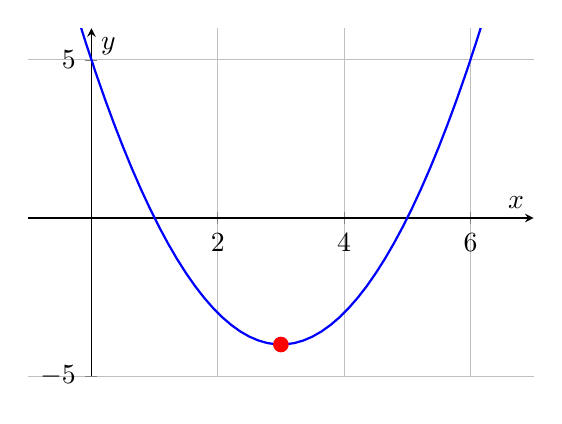
\begin{tikzpicture}
\begin{axis}[
    axis lines=middle,
    xlabel=$x$,
    ylabel=$y$,
    xmin=-1, xmax=7,
    ymin=-5, ymax=6,
    grid=major,
    width=8cm,
    height=6cm
]
\addplot[blue, thick, domain=-0.5:6.5, samples=50] {x^2 - 6*x + 5};
\node[circle,fill=red,inner sep=2pt] at (axis cs:3,-4) {};
\end{axis}
\end{tikzpicture}
\end{center}
\end{solution}

\subsection{Polynomial Graphs}

\begin{exercise}
For $P(x) = -(x + 2)(x - 1)^2(x - 3)$, determine:
\begin{enumerate}[label=(\alph*)]
    \item The degree
    \item End behavior
    \item All roots and their multiplicities
    \item Behavior at each root (cross or bounce)
    \item The $y$-intercept
\end{enumerate}
\end{exercise}

\begin{solution}
\begin{enumerate}[label=(\alph*)]
    \item Degree: $1 + 2 + 1 = \boxed{4}$

    \item Degree 4 (even), leading coefficient negative:

    \textbf{Both ends go to $-\infty$}

    \item Roots:
    \begin{itemize}
        \item $x = -2$ (multiplicity 1)
        \item $x = 1$ (multiplicity 2)
        \item $x = 3$ (multiplicity 1)
    \end{itemize}

    \item Behavior:
    \begin{itemize}
        \item $x = -2$: crosses (odd multiplicity)
        \item $x = 1$: bounces (even multiplicity)
        \item $x = 3$: crosses (odd multiplicity)
    \end{itemize}

    \item $P(0) = -(2)(1)(-3) = 6$

    $y$-intercept: $\boxed{(0, 6)}$
\end{enumerate}
\end{solution}

%=============================================================================
\section{Week 4: Functions and Graphs}
%=============================================================================

\subsection{Domain and Range}

\begin{exercise}
Find the domain of each function:
\begin{enumerate}[label=(\alph*)]
    \item $f(x) = x^2 - 4x + 3$
    \item $g(x) = \frac{1}{x - 5}$
    \item $h(x) = \sqrt{x + 3}$
    \item $k(x) = \frac{x}{\sqrt{2x - 6}}$
\end{enumerate}
\end{exercise}

\begin{solution}
\begin{enumerate}[label=(\alph*)]
    \item Polynomial: Domain = $\boxed{(-\infty, \infty)}$ or $\mathbb{R}$

    \item Undefined when $x - 5 = 0$: Domain = $\boxed{(-\infty, 5) \cup (5, \infty)}$

    \item Requires $x + 3 \geq 0$: Domain = $\boxed{[-3, \infty)}$

    \item Requires $2x - 6 > 0$ (strict, since in denominator):

    $x > 3$: Domain = $\boxed{(3, \infty)}$
\end{enumerate}
\end{solution}

\begin{exercise}
From the graph of $f(x) = -x^2 + 4$, determine:
\begin{enumerate}[label=(\alph*)]
    \item The domain
    \item The range
    \item Intervals where $f$ is increasing
    \item Intervals where $f$ is decreasing
\end{enumerate}
\end{exercise}

\begin{solution}
The function $f(x) = -x^2 + 4$ is a downward parabola with vertex at $(0, 4)$.
\begin{enumerate}[label=(\alph*)]
    \item Domain: $\boxed{(-\infty, \infty)}$
    \item Range: $\boxed{(-\infty, 4]}$ (maximum at vertex)
    \item Increasing: $\boxed{(-\infty, 0)}$
    \item Decreasing: $\boxed{(0, \infty)}$
\end{enumerate}
\end{solution}

\subsection{Function Operations and Composition}

\begin{exercise}
Let $f(x) = x^2 + 1$ and $g(x) = 2x - 3$. Find:
\begin{enumerate}[label=(\alph*)]
    \item $(f + g)(x)$
    \item $(f - g)(x)$
    \item $(f \cdot g)(2)$
    \item $(f/g)(x)$ and its domain
\end{enumerate}
\end{exercise}

\begin{solution}
\begin{enumerate}[label=(\alph*)]
    \item $(f + g)(x) = x^2 + 1 + 2x - 3 = \boxed{x^2 + 2x - 2}$

    \item $(f - g)(x) = x^2 + 1 - (2x - 3) = \boxed{x^2 - 2x + 4}$

    \item $f(2) = 5$, $g(2) = 1$

    $(f \cdot g)(2) = 5 \times 1 = \boxed{5}$

    \item $(f/g)(x) = \frac{x^2 + 1}{2x - 3}$

    Domain: $2x - 3 \neq 0 \Rightarrow x \neq \frac{3}{2}$

    Domain: $\boxed{(-\infty, \frac{3}{2}) \cup (\frac{3}{2}, \infty)}$
\end{enumerate}
\end{solution}

\begin{exercise}
Let $f(x) = x^2$ and $g(x) = x + 4$. Find:
\begin{enumerate}[label=(\alph*)]
    \item $(f \circ g)(x)$
    \item $(g \circ f)(x)$
    \item $(f \circ g)(2)$
    \item $(g \circ f)(-3)$
\end{enumerate}
\end{exercise}

\begin{solution}
\begin{enumerate}[label=(\alph*)]
    \item $(f \circ g)(x) = f(g(x)) = f(x + 4) = (x + 4)^2 = \boxed{x^2 + 8x + 16}$

    \item $(g \circ f)(x) = g(f(x)) = g(x^2) = x^2 + 4 = \boxed{x^2 + 4}$

    \item $(f \circ g)(2) = (2 + 4)^2 = 36$ or use formula: $4 + 16 + 16 = \boxed{36}$

    \item $(g \circ f)(-3) = (-3)^2 + 4 = 9 + 4 = \boxed{13}$
\end{enumerate}
\end{solution}

\begin{exercise}
Let $f(x) = \sqrt{x}$ and $g(x) = x - 5$. Find $(f \circ g)(x)$ and its domain.
\end{exercise}

\begin{solution}
$(f \circ g)(x) = f(g(x)) = f(x - 5) = \sqrt{x - 5}$

Domain: Need $x - 5 \geq 0$, so $x \geq 5$

Domain: $\boxed{[5, \infty)}$
\end{solution}

\subsection{Transformations}

\begin{exercise}
Starting with $f(x) = x^2$, describe the transformations to obtain each function:
\begin{enumerate}[label=(\alph*)]
    \item $g(x) = x^2 + 3$
    \item $h(x) = (x - 2)^2$
    \item $k(x) = -x^2$
    \item $m(x) = (x + 1)^2 - 4$
\end{enumerate}
\end{exercise}

\begin{solution}
\begin{enumerate}[label=(\alph*)]
    \item $g(x) = x^2 + 3$: \textbf{Shift up 3 units}

    \item $h(x) = (x - 2)^2$: \textbf{Shift right 2 units}

    \item $k(x) = -x^2$: \textbf{Reflect across $x$-axis}

    \item $m(x) = (x + 1)^2 - 4$: \textbf{Shift left 1 unit, then down 4 units}

    Vertex moves from $(0, 0)$ to $(-1, -4)$
\end{enumerate}
\end{solution}

\begin{exercise}
The graph of $f(x) = |x|$ is transformed to create $g(x) = -|x - 3| + 2$. Describe all transformations and identify the vertex of $g$.
\end{exercise}

\begin{solution}
Starting with $f(x) = |x|$ (V-shape with vertex at origin):

\begin{enumerate}
    \item $|x - 3|$: Shift \textbf{right 3 units}
    \item $-|x - 3|$: \textbf{Reflect across $x$-axis} (V flips to $\Lambda$)
    \item $-|x - 3| + 2$: Shift \textbf{up 2 units}
\end{enumerate}

\textbf{Vertex of $g$: $(3, 2)$}

The graph is an inverted V-shape opening downward.
\end{solution}

\subsection{Continuity}

\begin{exercise}
Identify whether each function is continuous on its domain. If not, describe the type of discontinuity.
\begin{enumerate}[label=(\alph*)]
    \item $f(x) = x^3 - 2x + 1$
    \item $g(x) = \frac{1}{x}$
    \item $h(x) = \frac{x^2 - 4}{x - 2}$
\end{enumerate}
\end{exercise}

\begin{solution}
\begin{enumerate}[label=(\alph*)]
    \item $f(x) = x^3 - 2x + 1$: \textbf{Continuous everywhere}

    (All polynomials are continuous on $\mathbb{R}$)

    \item $g(x) = \frac{1}{x}$: \textbf{Discontinuous at $x = 0$}

    Type: \textbf{Infinite discontinuity} (vertical asymptote)

    \item $h(x) = \frac{x^2 - 4}{x - 2} = \frac{(x-2)(x+2)}{x - 2} = x + 2$ for $x \neq 2$

    \textbf{Discontinuous at $x = 2$}

    Type: \textbf{Removable discontinuity} (hole at $(2, 4)$)
\end{enumerate}
\end{solution}

\end{document}
